% !TeX root = ../../thesis.tex
\chapter{Advanced model with kinetics}\label{ch:kinetics}


\begin{shaded}
This chapter is based on prepared manuscript to be submitted to  \textit{npj Computational Materials}:\\
M. Barzegari, C. Wang, S.V. Lamaka, G. Zavodszky, and L. Geris, ``Interface-coupled multiphysics computational modeling of local pH changes during the biodegradation of magnesium biomaterials,'' will be submitted to \textit{npj Computational Materials}.
\end{shaded}

\section{Introduction}


\section{Results}

\begin{figure}[h]
\centering
\medskip
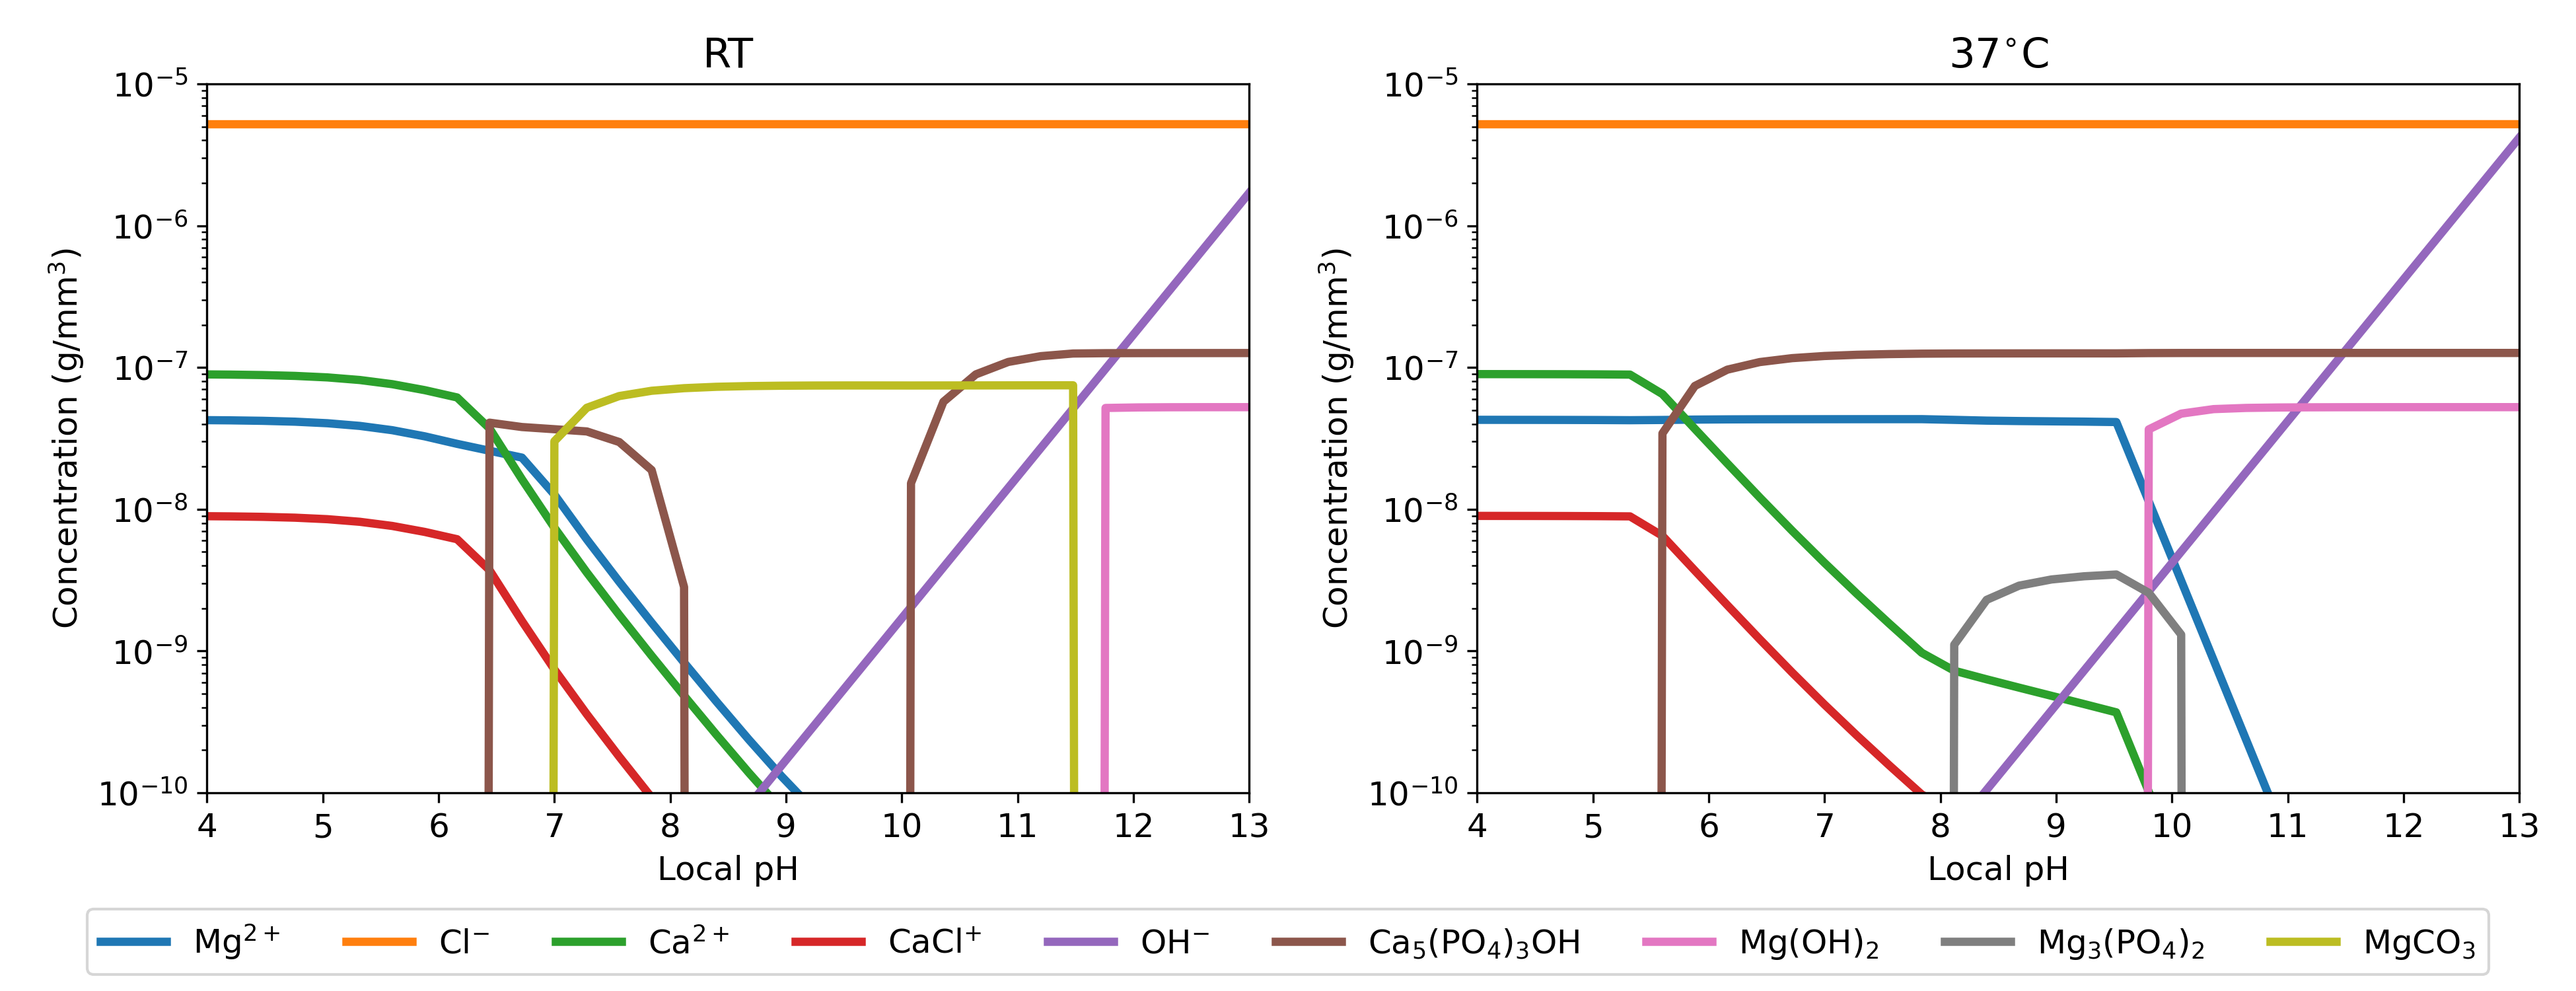
\includegraphics[width=\textwidth]{medusa_profiles.png}
\caption[Hydra-Medusa software output for given experiment conditions]{Selected components from the Hydra-Medusa software output for given experiment conditions} \label{fig:kinetics_medusa_profiles}
\end{figure}

\begin{figure}[h]
\centering
\medskip
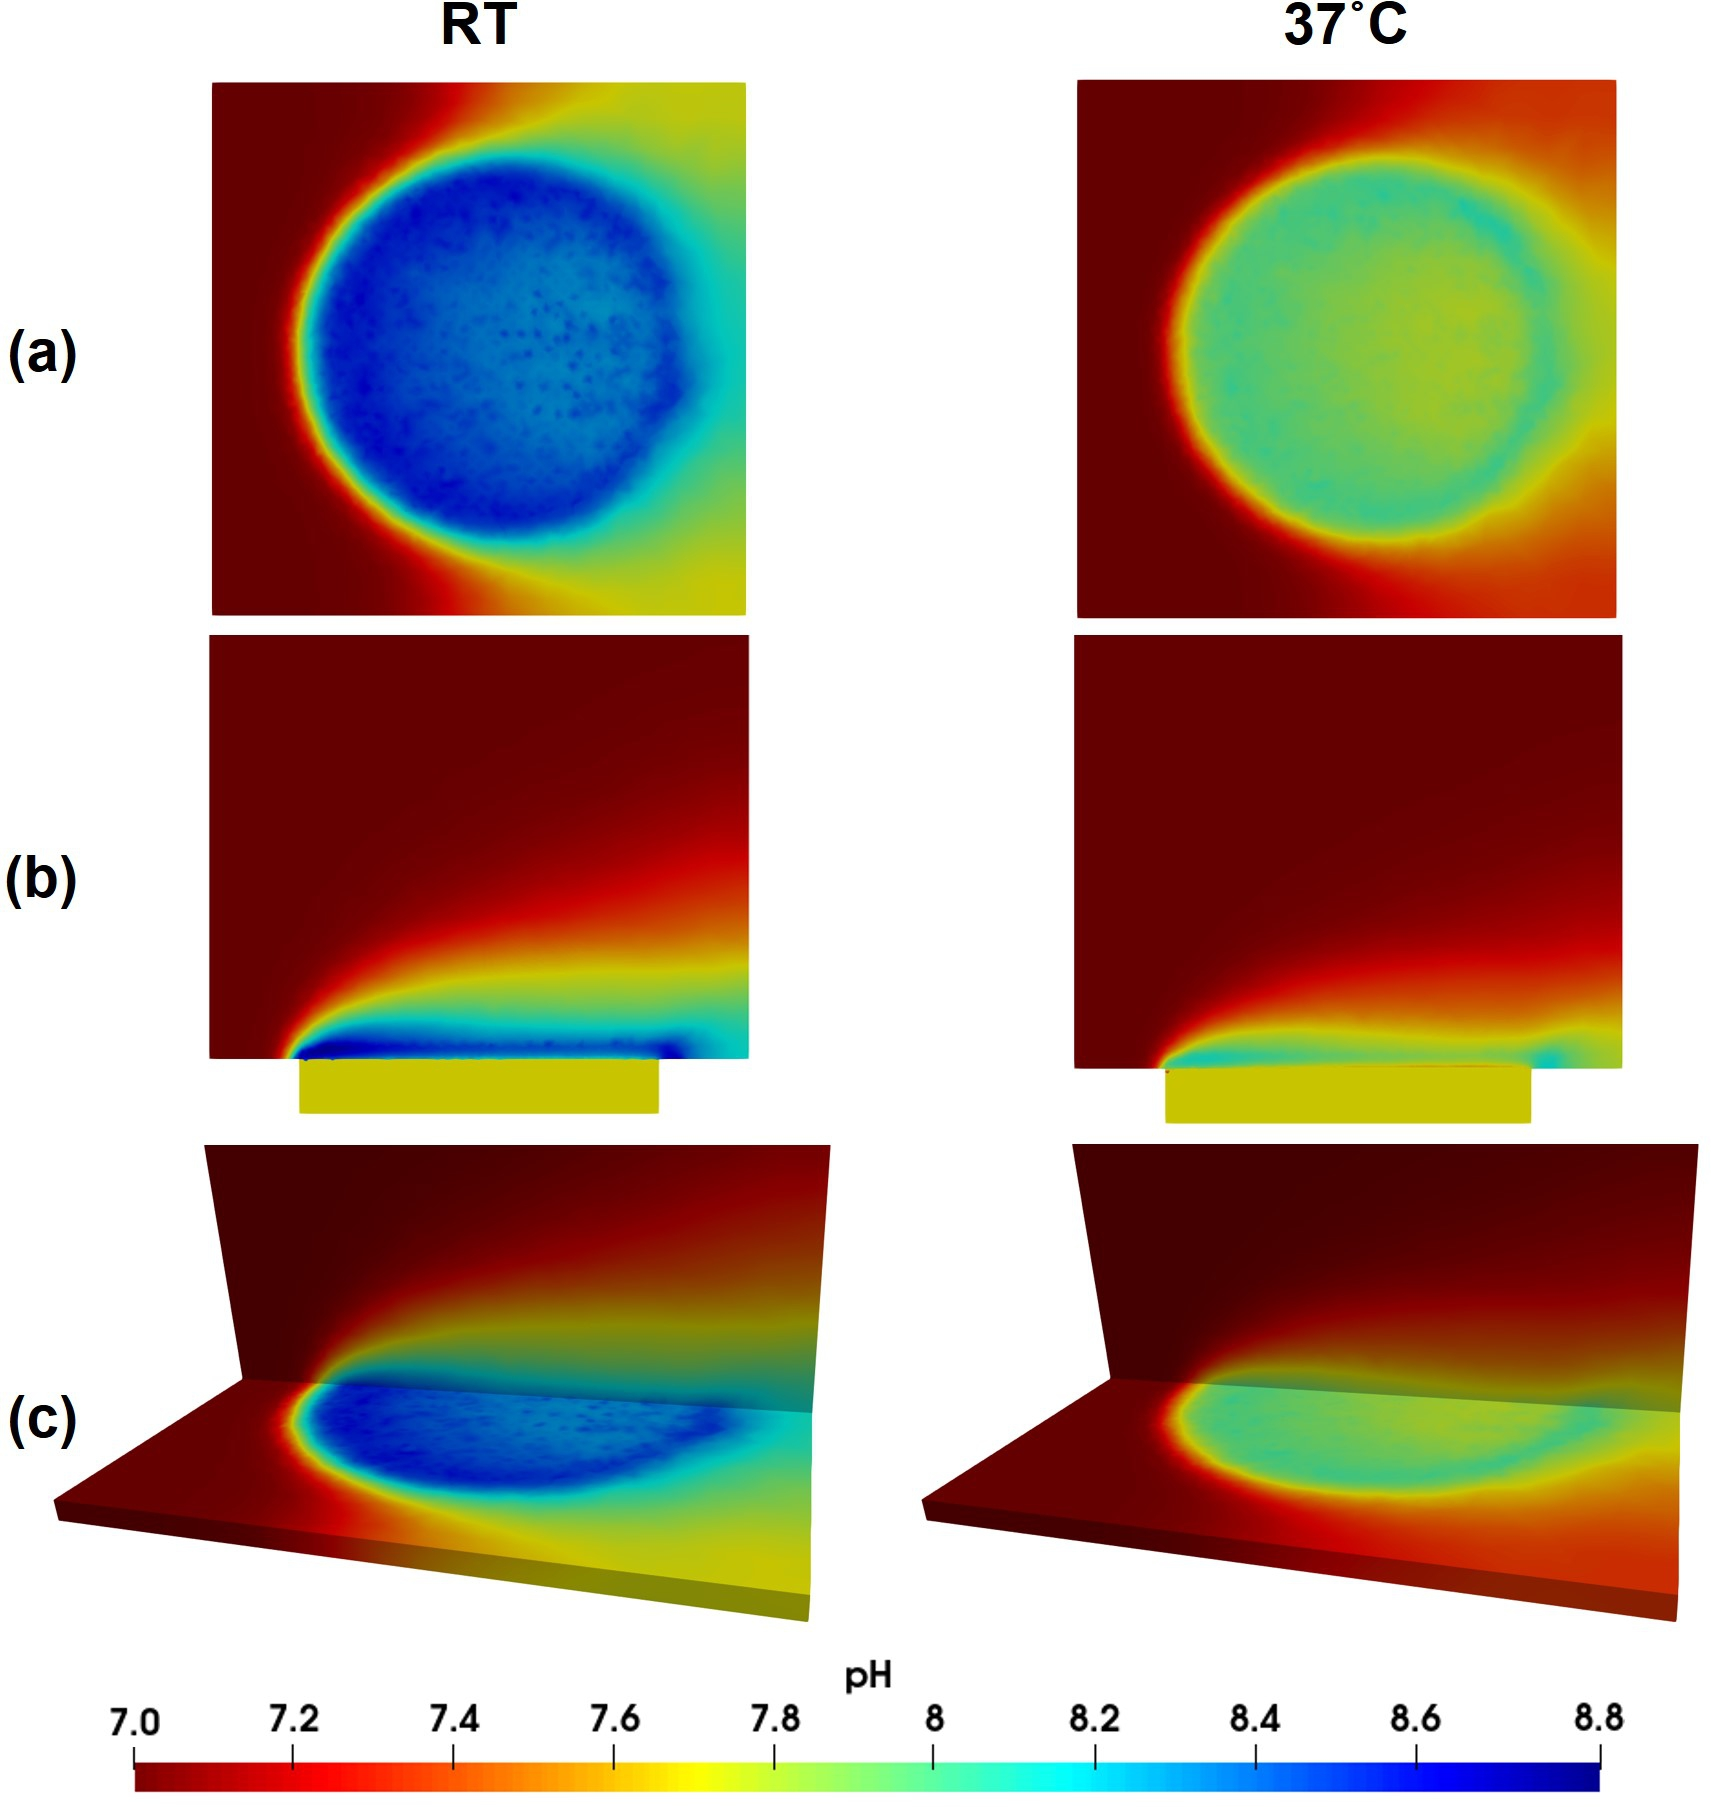
\includegraphics[width=\textwidth]{local_ph_visual.jpg}
\caption[Simulation results for local pH predictions]{Simulation results for local pH predictions} \label{fig:kinetics_local_ph_visual}
\end{figure}

\begin{figure}[h]
\centering
\medskip
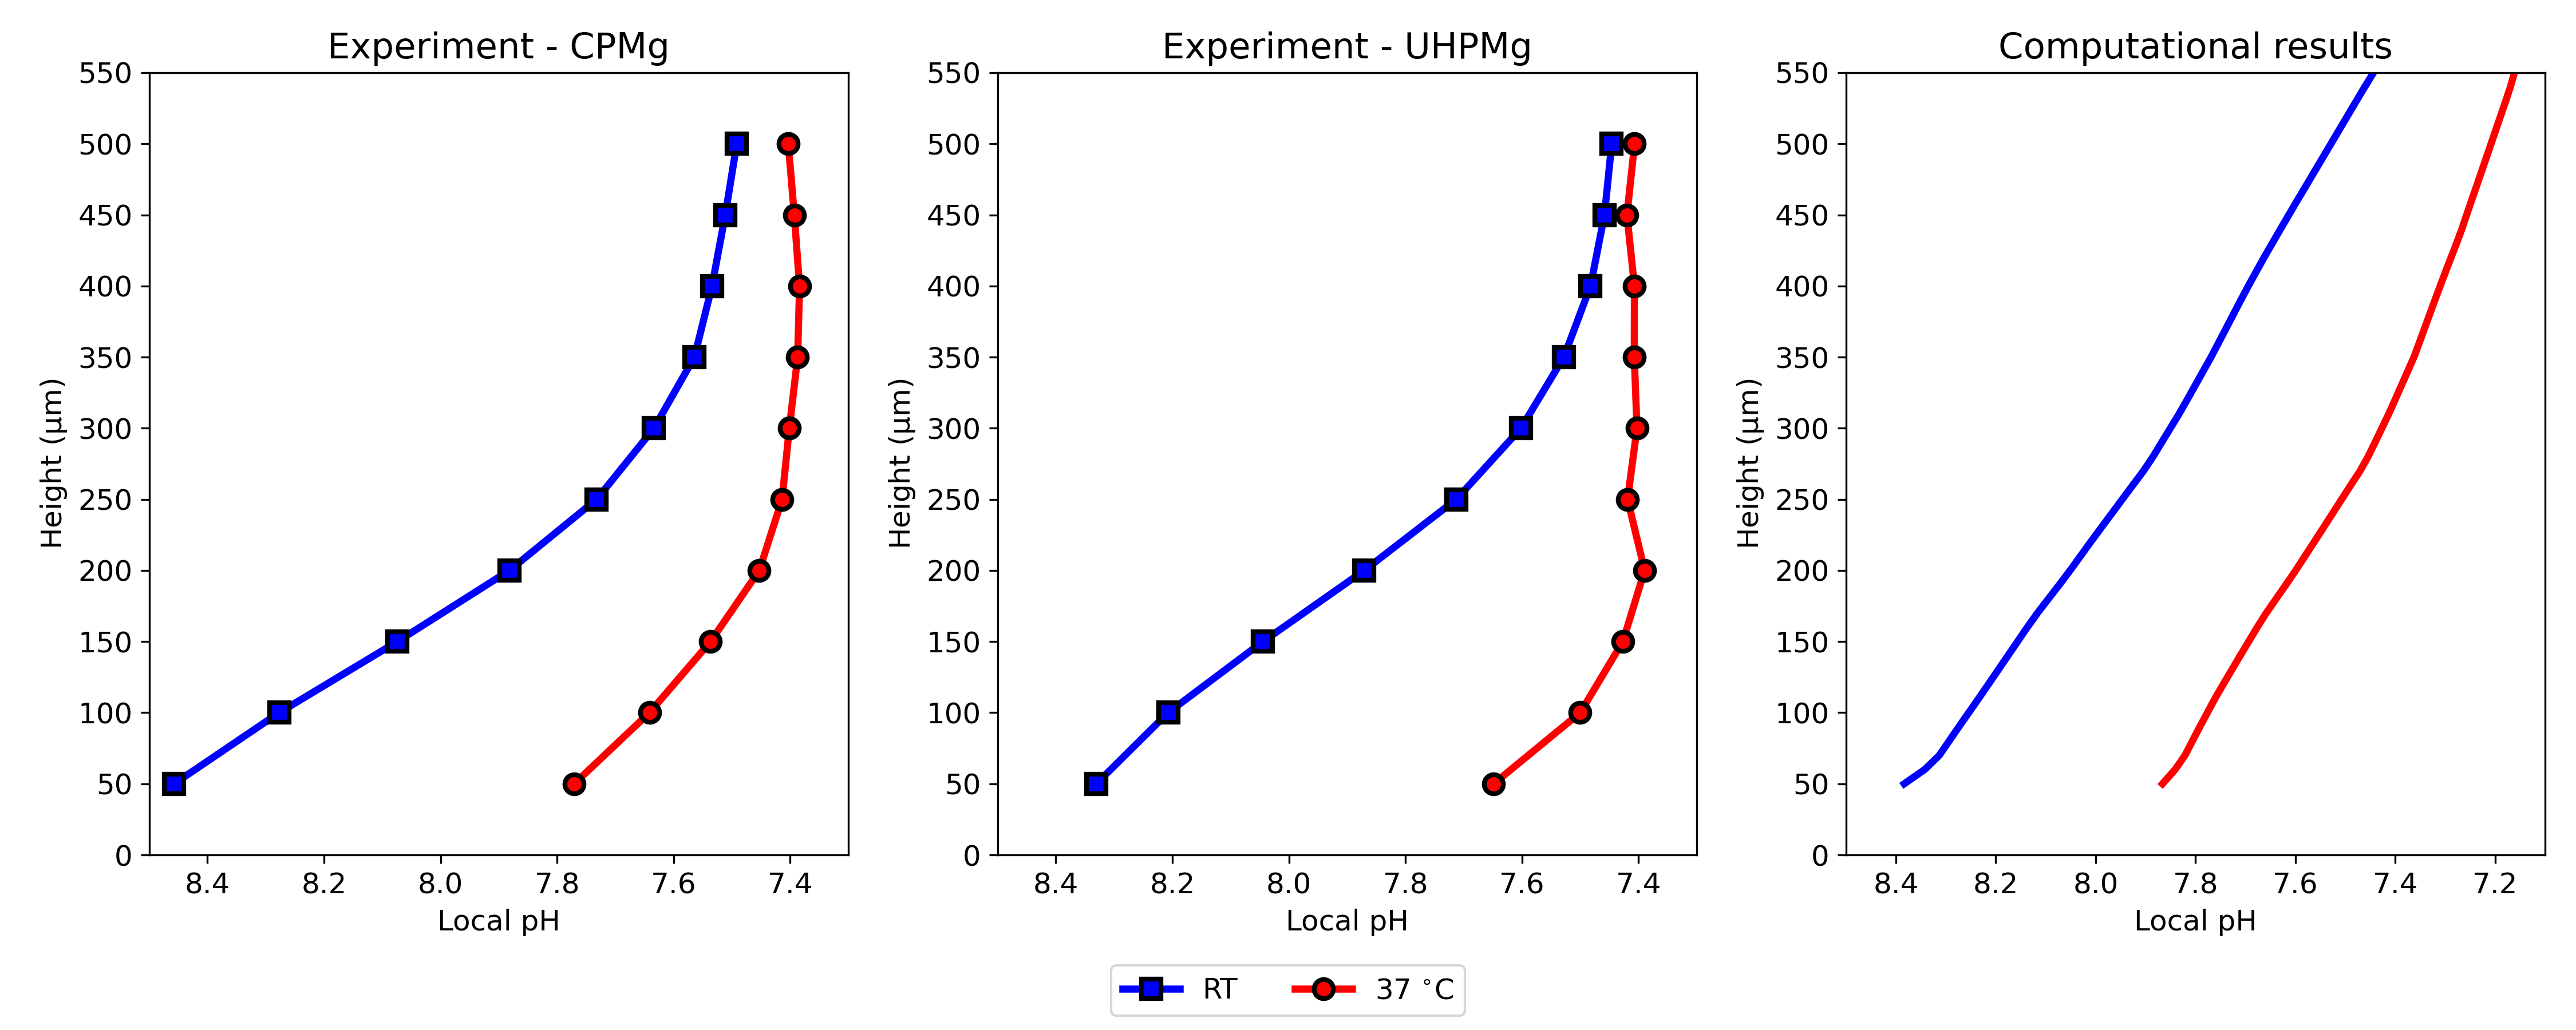
\includegraphics[width=\textwidth]{vertical_profile.png}
\caption[Comparing computational and experimental vertical pH profile]{Comparing computational and experimental vertical pH profile} \label{fig:kinetics_vertical_profile}
\end{figure}

\begin{figure}[h]
\centering
\medskip
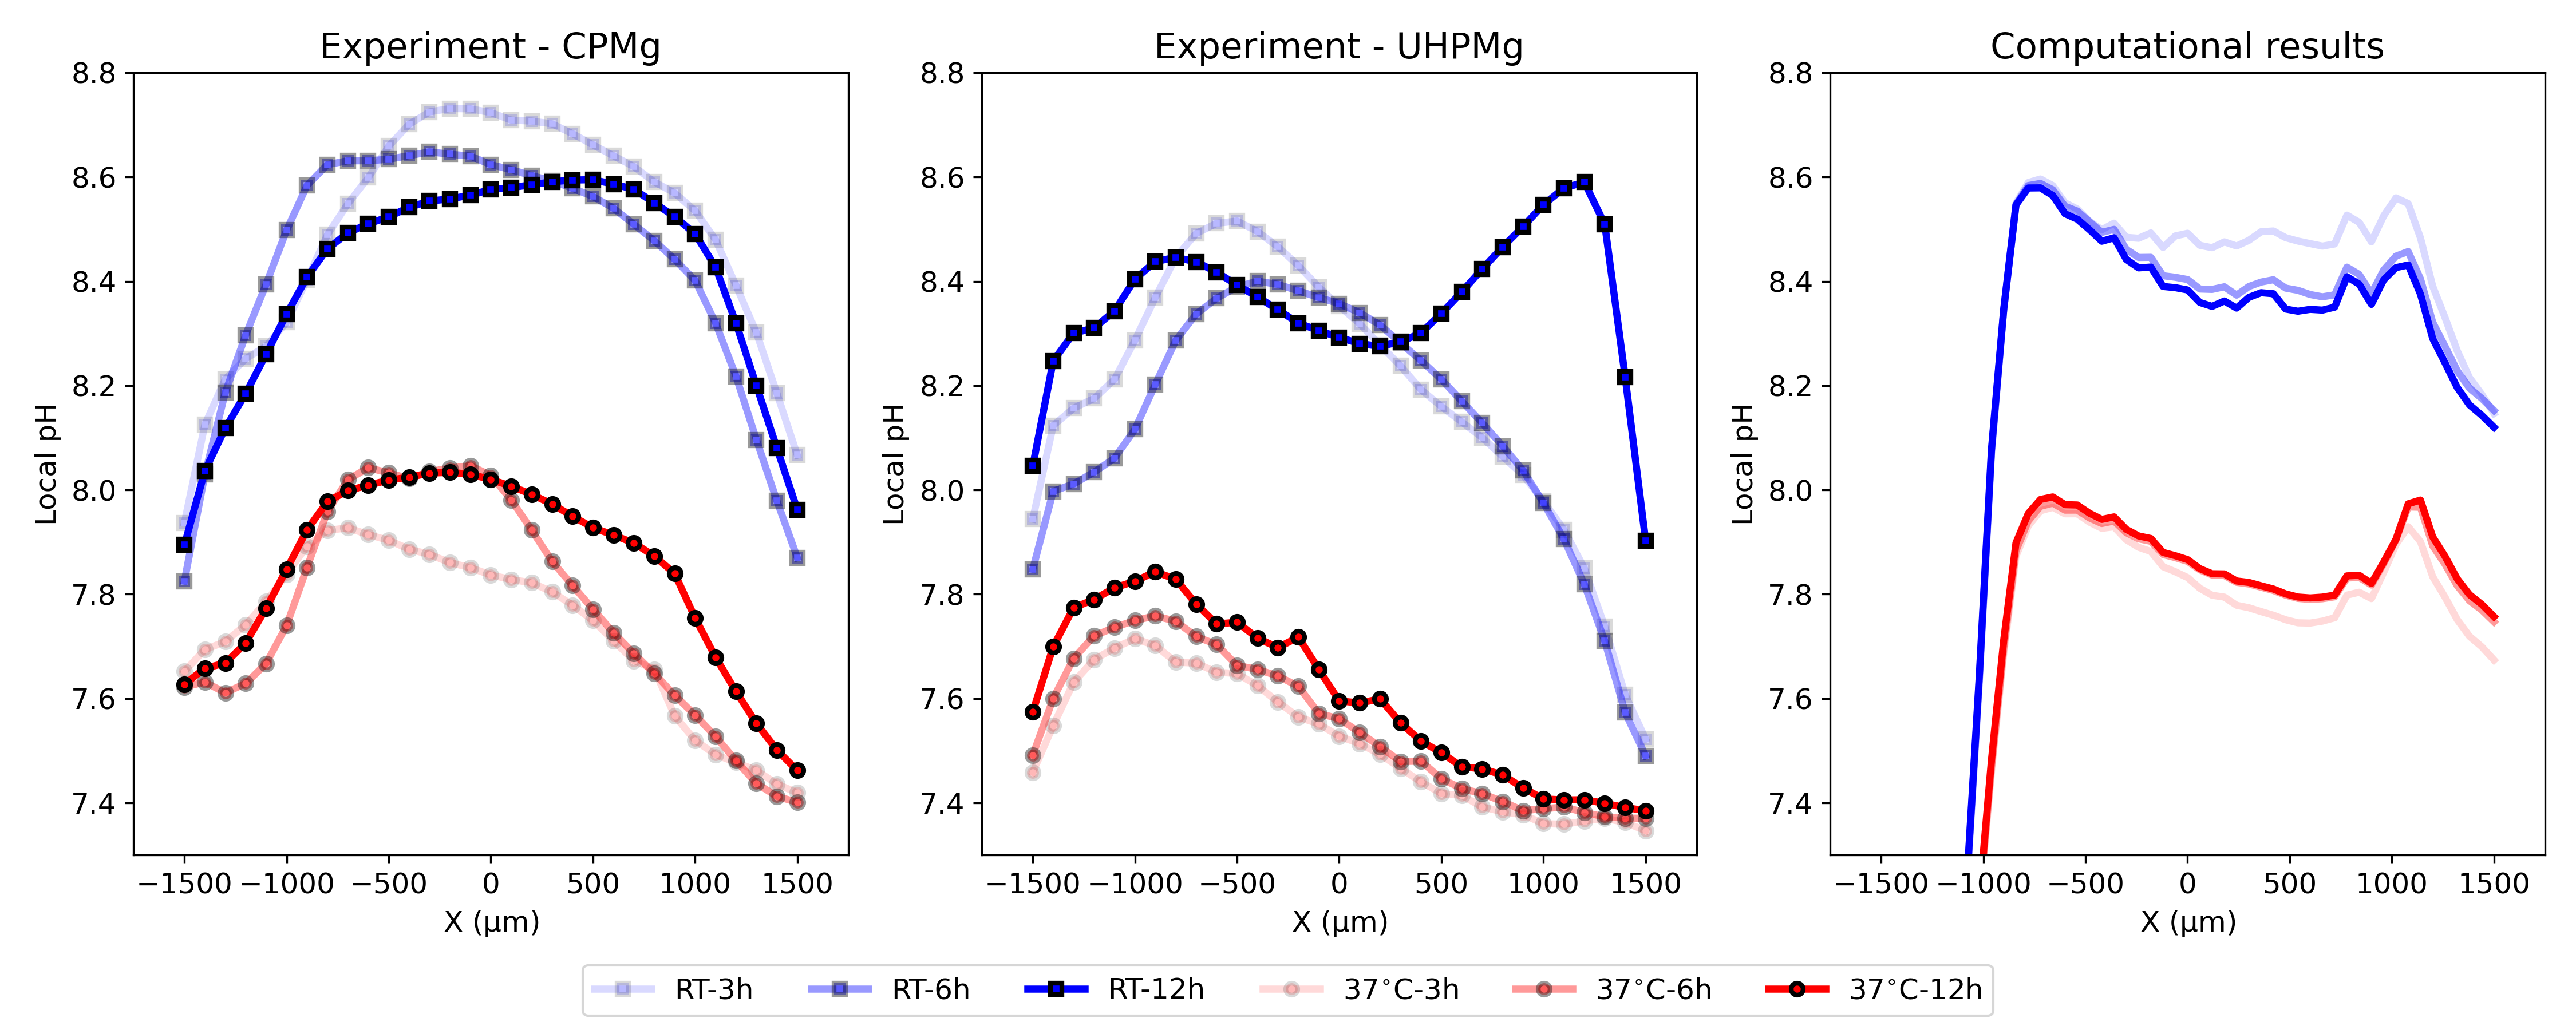
\includegraphics[width=\textwidth]{line_scans.png}
\caption[Comparing computational and experimental horizontal line scans for  local pH]{Comparing computational and experimental horizontal line scans for  local pH} \label{fig:kinetics_line_scans}
\end{figure}

\section{Discussion}

\section{Methods}

\begin{figure}[h]
\centering
\medskip
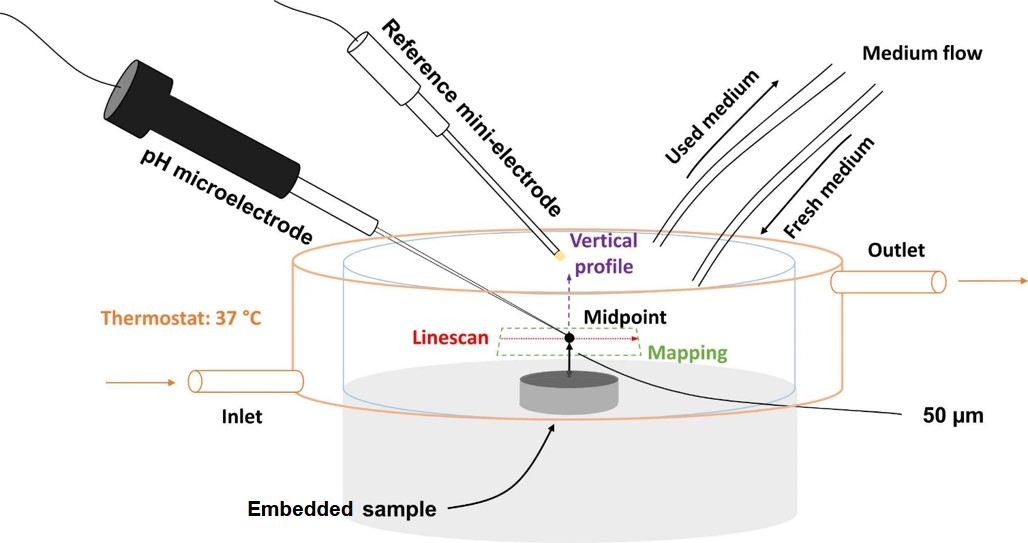
\includegraphics[width=0.8\textwidth]{setup.jpg}
\caption[Experimental setup for validating the coupled biodegradation model]{Experimental setup for validating the coupled biodegradation model} \label{fig:kinetics_setup}
\end{figure}


\begin{figure}[h]
\centering
\medskip
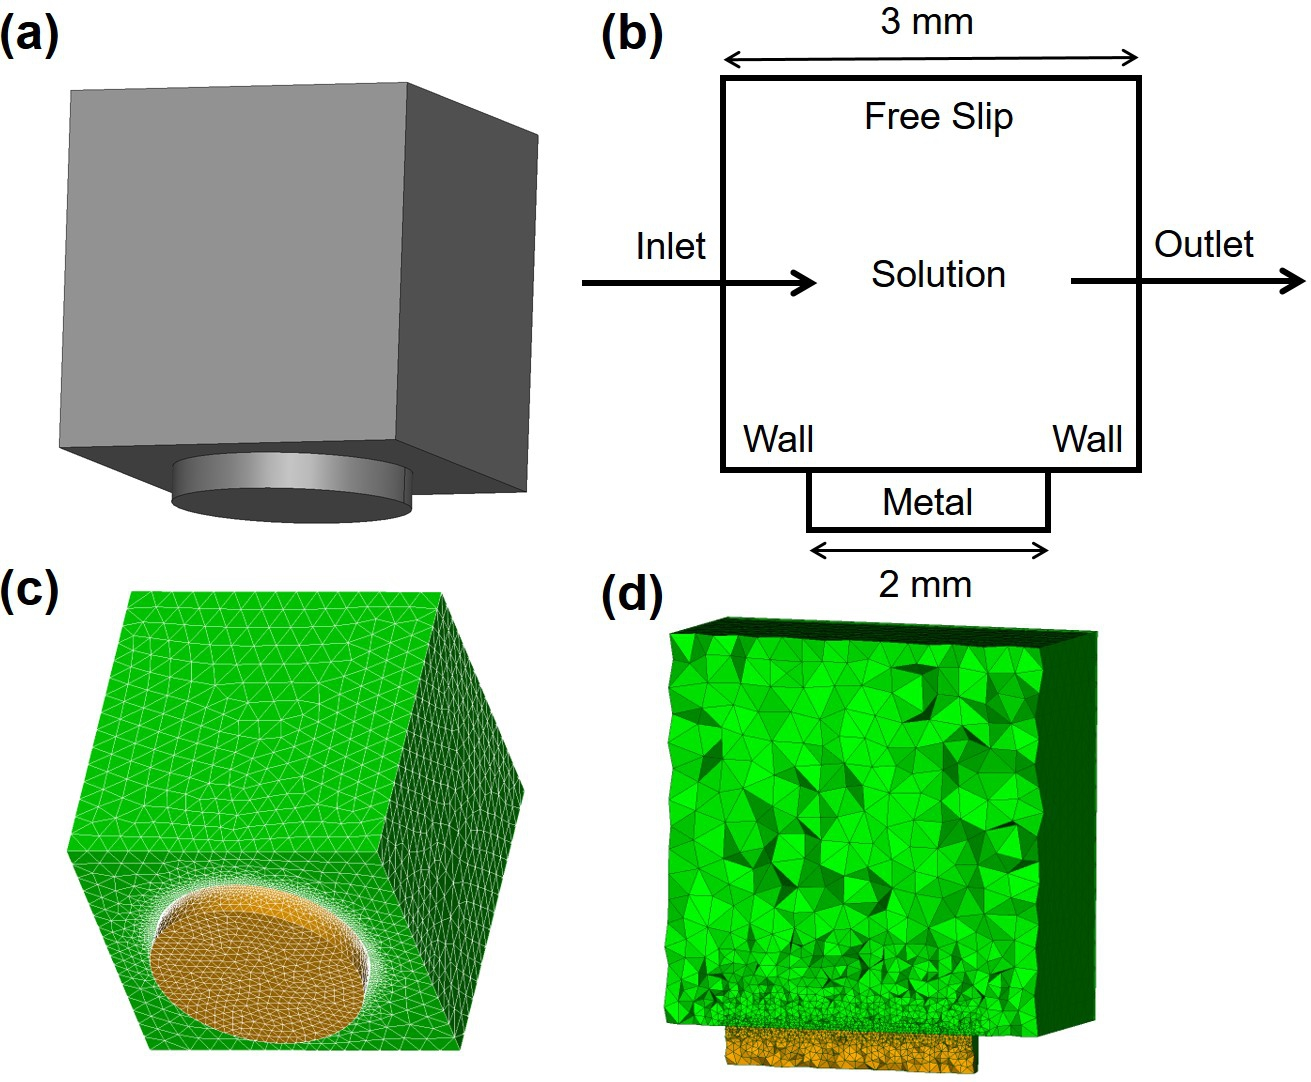
\includegraphics[width=\textwidth]{model_setup.jpg}
\caption[Computational model setup for local pH simulations]{Computational model setup for local pH simulations} \label{fig:kinetics_model_setup}
\end{figure}



\section{Data Availability}

The data used in the paper are available from the authors upon request.

\section{Code Availability}
The source code of the programs used in this paper is available from the authors upon request.


\section{Acknowledgements}

\section{Author Contributions}

\section{Competing Interests}


%%%%%%%%%%%%%%%%%%%%%%%%%%%%%%%%%%%%%%%%%%%%%%%%%%
% Keep the following \cleardoublepage at the end of this file, 
% otherwise \includeonly includes empty pages.
\cleardoublepage

